In this lab work I study the design of digital systems using one of the most common hardware description languages (HDL), Verilog (the other is VHL).

Using the Verilog language it is intended to implement in FPGA a state machine to control a washing machine. The board I use is the Basys 2 Spartan-3E FPGA Trainer Board.

I started by drawing the states and transitions diagram of \autoref{fig:diagram}, detailing the intended operation for the state machine, and it was through this diagram that I wrote the code that was implemented on the board.

\begin{figure}[H]
	\centering
	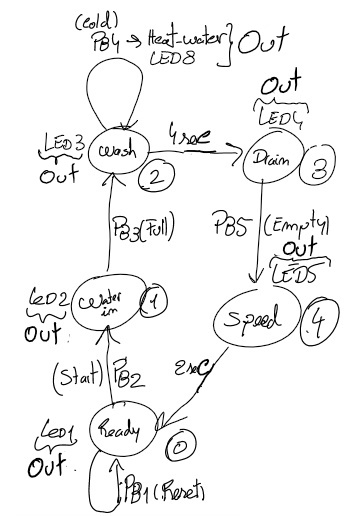
\includegraphics[width=.60\textwidth]{img/diagram}
	\caption{Finite state machine to be implemented}
	\label{fig:diagram}
\end{figure}

Once the desired implementation is defined, I developed the verilog code, as presented in the following section

